\chapter{Results}\label{chap:results}
\section{Simulation Scenarios}
\label{subsec:sim_scenarios}

To comprehensively evaluate the closed-loop performance of the adaptive MPC framework and its velocity-dependent weight scheduling strategy, six distinct simulation scenarios are defined. These test cases are carefully selected to excite the suspension system across a broad spectrum of operating conditions, encompassing both deterministic resonant frequencies and stochastic road roughness.

The six scenarios are defined in the following order:

\begin{itemize}
\item \textbf{Scenario 1: Sinusoidal input (\SI{0.03}{\metre} amplitude at \SI{1.3}{\hertz}).} This deterministic input is specifically designed to continuously excite the sprung mass (chassis) at its natural resonance frequency. It provides a worst-case scenario for evaluating ride comfort and the controller's ability to prevent excessive low-frequency heave motions.
\begin{figure}[H]
    \centering
    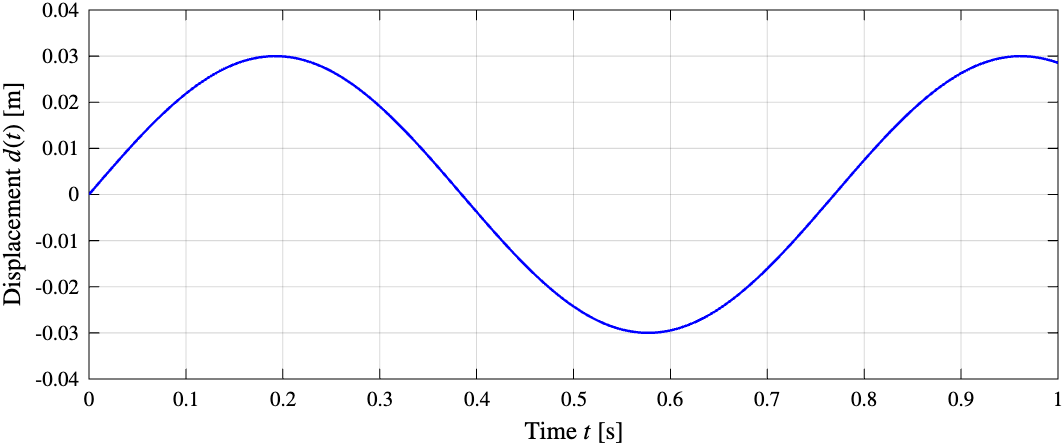
\includegraphics[width=0.6\linewidth]{Results/Graphs/Road Profiles/Scenario 1.png}
    \caption{Sinusoidal road profile of frequency = 1.3Hz}
    \label{fig:Road13}
\end{figure}
\item \textbf{Scenario 2: Sinusoidal input (\SI{0.03}{\metre} amplitude at \SI{10.9}{\hertz}).} This high-frequency deterministic input targets the unsprung mass (wheel and tyre) resonance frequency. It serves as a stringent test for the road-holding objective, evaluating the controller's capacity to suppress wheel hop and prevent tyre lift-off under severe resonant excitation.
\begin{figure}[H]
    \centering
    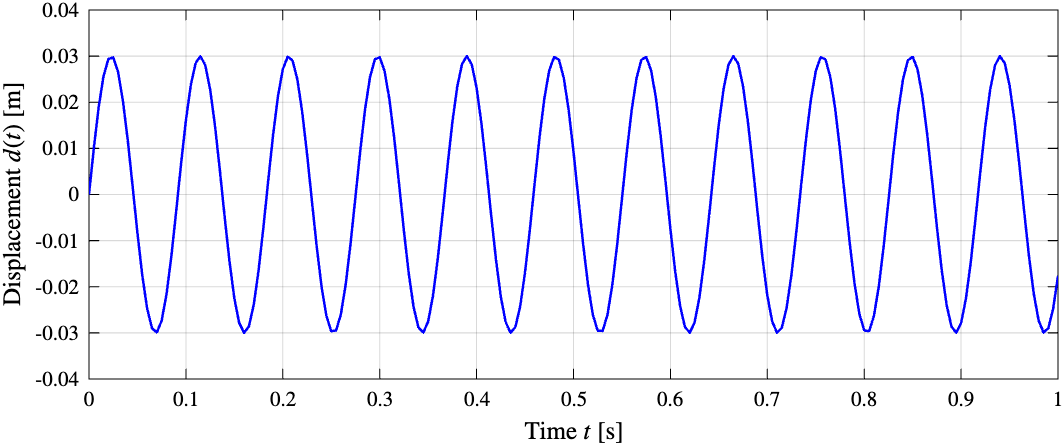
\includegraphics[width=0.6\linewidth]{Results/Graphs/Road Profiles/Scenario 2.png}
    \caption{Sinusoidal road profile of frequency = 10.9Hz}
    \label{fig:Road109}
\end{figure}
\item \textbf{Scenario 3: Class~B road at \SI{120}{\kilo\metre\per\hour}.} This highway driving scenario evaluates the pure performance boundary of the adaptive scheduler. At this high velocity, the controller overwhelmingly prioritizes the minimization of tyre dynamic loads to ensure continuous road contact and vehicle stability.
\begin{figure}[H]
    \centering
    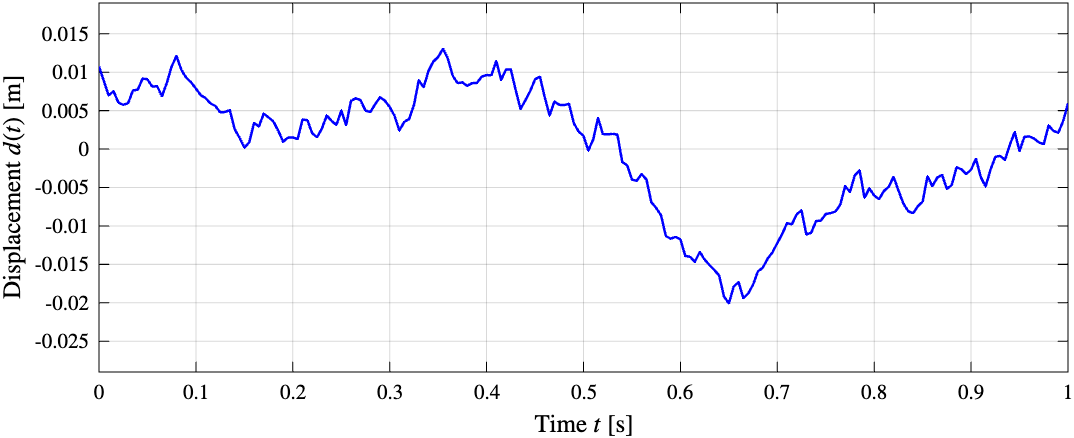
\includegraphics[width=0.6\linewidth]{Results/Graphs/Road Profiles/Scenario 3.png}
    \caption{Class B road at 120km/h}
    \label{fig:RoadBH}
\end{figure}
\item \textbf{Scenario 4: Class~B road at \SI{40}{\kilo\metre\per\hour}.} This represents typical urban driving on a good quality surface. The dynamic tyre forces are naturally low, allowing the controller to heavily penalize body acceleration and maximize passenger comfort.
\begin{figure}[H]
    \centering
    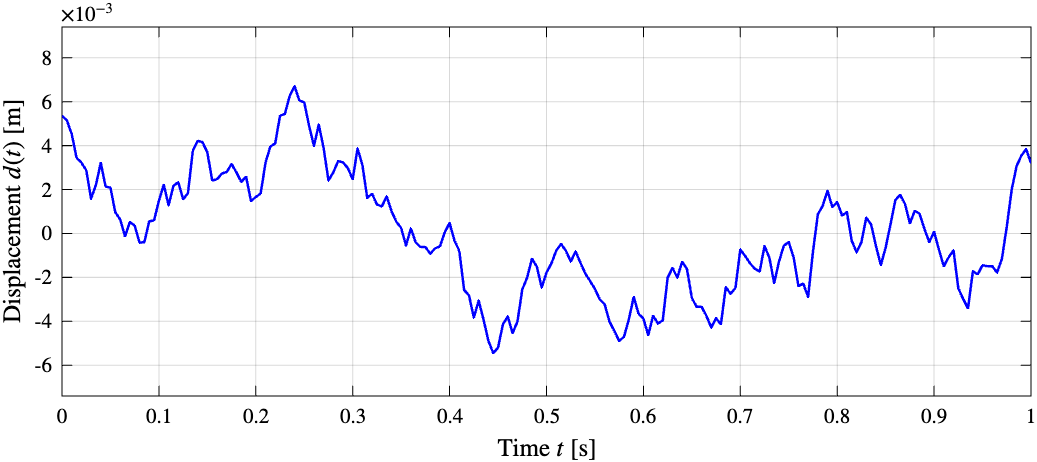
\includegraphics[width=0.6\linewidth]{Results/Graphs/Road Profiles/Scenario 4.png}
    \caption{Class B road at 40km/h}
    \label{fig:RoadBL}
\end{figure}
\item \textbf{Scenario 5: Class~D road at \SI{60}{\kilo\metre\per\hour}.} Operating on a poor quality road, this increased velocity pushes the MPC weight scheduler past the inflection point ($v_{mid} = \SI{50}{\kilo\metre\per\hour}$). This tests the controller's ability to manage high-amplitude disturbances while shifting priority toward road holding and dynamic safety.
\begin{figure}[H]
    \centering
    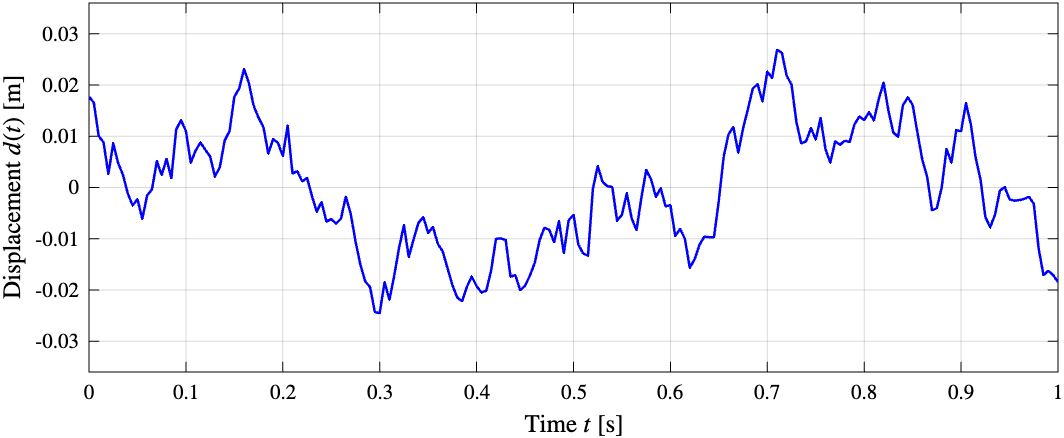
\includegraphics[width=0.6\linewidth]{Results/Graphs/Road Profiles/Scenario 5.png}
    \caption{Class D road at 60km/h}
    \label{fig:RoadDH}
\end{figure}
\item \textbf{Scenario 6: Class~D road at \SI{40}{\kilo\metre\per\hour}.} This scenario represents driving on a poor quality road at a low speed. According to the adaptive scheduling strategy (\cref{subsec:mpc_scheduling}), the controller operates in a comfort-dominant regime, testing the system's ability to isolate the chassis from severe, low-speed irregularities.
\begin{figure}[H]
    \centering
    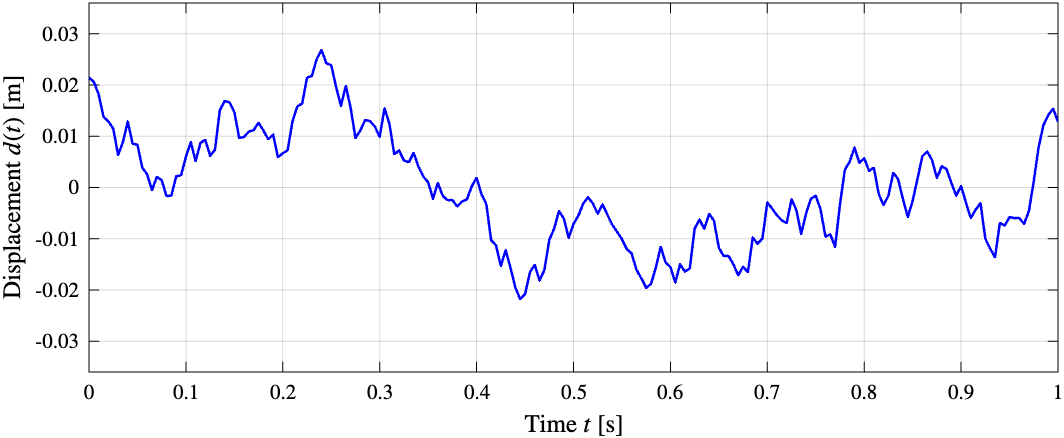
\includegraphics[width=0.6\linewidth]{Results/Graphs/Road Profiles/Scenario 6.png}
    \caption{Class D road at 40km/h}
    \label{fig:RoadDL}
\end{figure}
\end{itemize}

By subjecting the unified mechanical--electrical plant to this diverse set of disturbances, the robustness of the nested control architecture can be validated. The subsequent sections analyze the time-domain responses and performance metrics across these six scenarios, benchmarking the proposed adaptive MPC against passive suspension baselines.

\section{Reference Controller Performance}
The initial phase of the comparative analysis evaluates the theoretical reference forces generated by the high-level Model Predictive Control (MPC) and Hybrid Skyhook-Groundhook (HSG) algorithms. This comparison isolates the mathematical decision-making logic of the two controllers before accounting for the physical limitations of the electrical actuator. The objective is to highlight the fundamental operational differences between the algorithms, specifically examining how the MPC handles multi-objective constraints over a finite horizon compared to the unconstrained, memoryless formulation of the classical HSG strategy.

\subsection{Body Acceleration}
\begin{figure}[H]
    \centering
    
\includegraphics[width=0.75\linewidth]{Results/Graphs/Reference Comparison/BA13.png}
    \caption{Body Acceleration on sinusoidal road profile of frequency = 1.3Hz}
    \label{fig:BARef13}
\end{figure}
\begin{figure}[H]
    \centering
    
\includegraphics[width=0.75\linewidth]{Results/Graphs/Reference Comparison/BA109.png}
    \caption{Body Acceleration on sinusoidal road profile of frequency = 10.9Hz}
    \label{fig:BARef109}
\end{figure}
\begin{figure}[H]
    \centering
    
\includegraphics[width=0.75\linewidth]{Results/Graphs/Reference Comparison/BABH.png}
    \caption{Body Acceleration on class B road at 120km/h}
    \label{fig:BARefBH}
\end{figure}
\begin{figure}[H]
    \centering
    
\includegraphics[width=0.75\linewidth]{Results/Graphs/Reference Comparison/BABL.png}
    \caption{Body Acceleration on class B road at 40km/h}
    \label{fig:BARefBL}
\end{figure}
\begin{figure}[H]
    \centering
    
\includegraphics[width=0.75\linewidth]{Results/Graphs/Reference Comparison/BADH.png}
    \caption{Body Acceleration on class D road at 60km/h}
    \label{fig:BARefDH}
\end{figure}
\begin{figure}[H]
    \centering
    
\includegraphics[width=0.75\linewidth]{Results/Graphs/Reference Comparison/BADL.png}
    \caption{Body Acceleration on class D road at 40km/h}
    \label{fig:BARefDL}
\end{figure}

The theoretical reference data reveals distinct mathematical approaches between the two formulations. The standard HSG logic computes an unconstrained optimal force, inherently prioritizing the immediate, maximum attenuation of body acceleration. For instance, at the 1.3~Hz chassis resonance, the HSG targets an aggressive body acceleration RMS of $1.38\text{ m/s}^2$. The MPC algorithm, however, evaluates a multi-objective cost function over a finite prediction horizon, inherently balancing ride comfort against road holding and actuator smoothness. This holistic optimization results in a more conservative, yet highly stable, predicted body acceleration RMS of $2.08\text{ m/s}^2$. 

\begin{table}[H]
    \centering
    \caption{Theoretical Reference Metrics: Body Acceleration}
    \label{tab:ref_ba_metrics}
    \renewcommand{\arraystretch}{1.2}
    \begin{tabular}{lcc}
        \toprule
        \textbf{Scenario} & \textbf{HSG Ref RMS} [m/s$^2$] & \textbf{MPC Ref RMS} [m/s$^2$] \\
        \midrule
        1.3 Hz Sine      & 1.38 & 2.08 \\
        10.9 Hz Sine     & 12.00 & 12.93 \\
        Class B, 120 km/h & 0.93 & 2.55 \\
        Class B, 40 km/h  & 0.54 & 1.33 \\
        Class D, 60 km/h  & 2.65 & 7.18 \\
        Class D, 40 km/h  & 2.16 & 5.31 \\
        \bottomrule
    \end{tabular}
\end{table}

\subsection{Tyre Dynamic Load}
\begin{figure}[H]
    \centering
    
\includegraphics[width=0.75\linewidth]{Results/Graphs/Reference Comparison/RH13.png}
    \caption{Tyre Dynamic Load on sinusoidal road profile of frequency = 1.3Hz}
    \label{fig:RHRef13}
\end{figure}
\begin{figure}[H]
    \centering
    
\includegraphics[width=0.75\linewidth]{Results/Graphs/Reference Comparison/RH109.png}
    \caption{Tyre Dynamic Load on sinusoidal road profile of frequency = 10.9Hz}
    \label{fig:RHRef109}
\end{figure}
\begin{figure}[H]
    \centering
    
\includegraphics[width=0.75\linewidth]{Results/Graphs/Reference Comparison/RHBH.png}
    \caption{Tyre Dynamic Load on class B road at 120km/h}
    \label{fig:RHRefBH}
\end{figure}
\begin{figure}[H]
    \centering
    
\includegraphics[width=0.75\linewidth]{Results/Graphs/Reference Comparison/RHBL.png}
    \caption{Tyre Dynamic Load on class B road at 40km/h}
    \label{fig:RHRefBL}
\end{figure}
\begin{figure}[H]
    \centering
    
\includegraphics[width=0.75\linewidth]{Results/Graphs/Reference Comparison/RHDH.png}
    \caption{Tyre Dynamic Load on class D road at 60km/h}
    \label{fig:RHRefDH}
\end{figure}
\begin{figure}[H]
    \centering
    
\includegraphics[width=0.75\linewidth]{Results/Graphs/Reference Comparison/RHDL.png}
    \caption{Tyre Dynamic Load on class D road at 40km/h}
    \label{fig:RHRefDL}
\end{figure}

Regarding road-holding, the controllers demonstrate divergent priorities under high-frequency excitation. During the 10.9~Hz unsprung mass resonance, the MPC predicts a focused tyre dynamic load RMS of $953.5\text{ N}$. The HSG algorithm, which places less emphasis on unsprung mass displacement in this frequency band, computes a significantly larger theoretical tyre dynamic load RMS of $2740.6\text{ N}$. Similar prioritization trends are evident across the stochastic ISO profiles.

\begin{table}[H]
    \centering
    \caption{Theoretical Reference Metrics: Tyre Dynamic Load}
    \label{tab:ref_rh_metrics}
    \renewcommand{\arraystretch}{1.2}
    \begin{tabular}{lcc}
        \toprule
        \textbf{Scenario} & \textbf{HSG Ref RMS} [N] & \textbf{MPC Ref RMS} [N] \\
        \midrule
        1.3 Hz Sine      & 122.6 & 184.7 \\
        10.9 Hz Sine     & 2740.6 & 953.5 \\
        Class B, 120 km/h & 193.4 & 136.0 \\
        Class B, 40 km/h  & 111.8 & 80.0 \\
        Class D, 60 km/h  & 547.4 & 385.3 \\
        Class D, 40 km/h  & 447.0 & 319.8 \\
        \bottomrule
    \end{tabular}
\end{table}

\section{Effect of Power Converter Dynamics}
Following the evaluation of the reference generation, the analysis shifts to force actualization. This section examines the tracking performance of the inner-loop Sliding Mode Controller (SMC) when subjected to the reference signals commanded by both the MPC and HSG algorithms. The primary goal is to examine how the physical limitations of the electrical actuator—namely bandwidth limits and slew rate constraints—affect the translation of theoretical references into actualized forces.

\subsection{Body Acceleration}
\subsubsection{HSG}
\begin{figure}[H]
    \centering
    
\includegraphics[width=0.75\linewidth]{Results/Graphs/Force Actualization/HSG/BA13.png}
    \caption{Body Acceleration on sinusoidal road profile of frequency = 1.3Hz}
    \label{fig:BAActHSG13}
\end{figure}
\begin{figure}[H]
    \centering
    
\includegraphics[width=0.75\linewidth]{Results/Graphs/Force Actualization/HSG/BA109.png}
    \caption{Body Acceleration on sinusoidal road profile of frequency = 10.9Hz}
    \label{fig:BAActHSG109}
\end{figure}
\begin{figure}[H]
    \centering
    
\includegraphics[width=0.75\linewidth]{Results/Graphs/Force Actualization/HSG/BABH.png}
    \caption{Body Acceleration on class B road at 120km/h}
    \label{fig:BAActHSGBH}
\end{figure}
\begin{figure}[H]
    \centering
    
\includegraphics[width=0.75\linewidth]{Results/Graphs/Force Actualization/HSG/BABL.png}
    \caption{Body Acceleration on class B road at 40km/h}
    \label{fig:BAActHSGBL}
\end{figure}
\begin{figure}[H]
    \centering
    
\includegraphics[width=0.75\linewidth]{Results/Graphs/Force Actualization/HSG/BADH.png}
    \caption{Body Acceleration on class D road at 60km/h}
    \label{fig:BAActHSGDH}
\end{figure}
\begin{figure}[H]
    \centering
    
\includegraphics[width=0.75\linewidth]{Results/Graphs/Force Actualization/HSG/BADL.png}
    \caption{Body Acceleration on class D road at 40km/h}
    \label{fig:BAActHSGDL}
\end{figure}

\subsubsection{MPC}
\begin{figure}[H]
    \centering
    
\includegraphics[width=0.75\linewidth]{Results/Graphs/Force Actualization/MPC/BA13.png}
    \caption{Body Acceleration on sinusoidal road profile of frequency = 1.3Hz}
    \label{fig:BAActMPC13}
\end{figure}
\begin{figure}[H]
    \centering
    
\includegraphics[width=0.75\linewidth]{Results/Graphs/Force Actualization/MPC/BA109.png}
    \caption{Body Acceleration on sinusoidal road profile of frequency = 10.9Hz}
    \label{fig:BAActMPC109}
\end{figure}
\begin{figure}[H]
    \centering
    
\includegraphics[width=0.75\linewidth]{Results/Graphs/Force Actualization/MPC/BABH.png}
    \caption{Body Acceleration on class B road at 120km/h}
    \label{fig:BAActMPCBH}
\end{figure}
\begin{figure}[H]
    \centering
    
\includegraphics[width=0.75\linewidth]{Results/Graphs/Force Actualization/MPC/BABL.png}
    \caption{Body Acceleration on class B road at 40km/h}
    \label{fig:BAActMPCBL}
\end{figure}
\begin{figure}[H]
    \centering
    
\includegraphics[width=0.75\linewidth]{Results/Graphs/Force Actualization/MPC/BADH.png}
    \caption{Body Acceleration on class D road at 60km/h}
    \label{fig:BAActMPCDH}
\end{figure}
\begin{figure}[H]
    \centering
    
\includegraphics[width=0.75\linewidth]{Results/Graphs/Force Actualization/MPC/BADL.png}
    \caption{Body Acceleration on class D road at 40km/h}
    \label{fig:BAActMPCDL}
\end{figure}

When theoretical references are routed through the inner-loop SMC, the effect of physical and electrical constraints becomes evident. At the 1.3~Hz chassis resonance, the memoryless HSG reference requests severe instantaneous force variations that exceed the operational limits of the electrical actuator, causing the SMC to clip the input. Consequently, the actualized HSG body acceleration RMS diverges from its theoretical target by $82.0\%$ ($2.51\text{ m/s}^2$ vs. $1.38\text{ m/s}^2$). Conversely, the MPC architecture achieves perfect tracking at 1.3~Hz ($0.0\%$ error) because its predictive horizon and control increment penalties generate smooth, dynamically feasible reference trajectories that the actuator can safely reproduce.

On stochastic ISO profiles, the actuator's bandwidth limits impact both controllers in different ways. The HSG controller tracks its stochastic references closely ($\sim 0.9\%$ tracking error). The MPC, however, commands rapidly fluctuating, high-magnitude forces on stochastic surfaces that encounter the electrical actuator's slew rate limits. This inadvertently introduces an electrical smoothing effect, causing the MPC to achieve a lower actualized body acceleration RMS than theoretically predicted.

\begin{table}[H]
    \centering
    \caption{Force Actualization and Tracking Error: Body Acceleration}
    \label{tab:act_ba_metrics}
    \renewcommand{\arraystretch}{1.2}
    \begin{tabular}{lcccc}
        \toprule
        \textbf{Scenario} & \textbf{HSG Act. RMS} & \textbf{HSG Err [\%]} & \textbf{MPC Act. RMS} & \textbf{MPC Err [\%]} \\
        \midrule
        1.3 Hz Sine      & 2.51 m/s$^2$ & +82.0 & 2.08 m/s$^2$ & \phantom{-}0.0 \\
        10.9 Hz Sine     & 12.01 m/s$^2$& +0.1  & 12.42 m/s$^2$& -4.0 \\
        Class B, 120 km/h& 0.94 m/s$^2$ & +0.8  & 1.50 m/s$^2$ & -41.2 \\
        Class B, 40 km/h & 0.55 m/s$^2$ & +0.9  & 0.86 m/s$^2$ & -34.9 \\
        Class D, 60 km/h & 2.67 m/s$^2$ & +0.9  & 4.25 m/s$^2$ & -40.8 \\
        Class D, 40 km/h & 2.18 m/s$^2$ & +0.9  & 3.46 m/s$^2$ & -34.9 \\
        \bottomrule
    \end{tabular}
\end{table}

\subsection{Tyre Dynamic Load}
\subsubsection{HSG}
\begin{figure}[H]
    \centering
    
\includegraphics[width=0.75\linewidth]{Results/Graphs/Force Actualization/HSG/RH13.png}
    \caption{Tyre Dynamic Load on sinusoidal road profile of frequency = 1.3Hz}
    \label{fig:RHActHSG13}
\end{figure}
\begin{figure}[H]
    \centering
    
\includegraphics[width=0.75\linewidth]{Results/Graphs/Force Actualization/HSG/RH109.png}
    \caption{Tyre Dynamic Load on sinusoidal road profile of frequency = 10.9Hz}
    \label{fig:RHActHSG109}
\end{figure}
\begin{figure}[H]
    \centering
    
\includegraphics[width=0.75\linewidth]{Results/Graphs/Force Actualization/HSG/RHBH.png}
    \caption{Tyre Dynamic Load on class B road at 120km/h}
    \label{fig:RHActHSGBH}
\end{figure}
\begin{figure}[H]
    \centering
    
\includegraphics[width=0.75\linewidth]{Results/Graphs/Force Actualization/HSG/RHBL.png}
    \caption{Tyre Dynamic Load on class B road at 40km/h}
    \label{fig:RHActHSGBL}
\end{figure}
\begin{figure}[H]
    \centering
    
\includegraphics[width=0.75\linewidth]{Results/Graphs/Force Actualization/HSG/RHDH.png}
    \caption{Tyre Dynamic Load on class D road at 60km/h}
    \label{fig:RHActHSGDH}
\end{figure}
\begin{figure}[H]
    \centering
    
\includegraphics[width=0.75\linewidth]{Results/Graphs/Force Actualization/HSG/RHDL.png}
    \caption{Tyre Dynamic Load on class D road at 40km/h}
    \label{fig:RHActHSGDL}
\end{figure}

\subsubsection{MPC}
\begin{figure}[H]
    \centering
    
\includegraphics[width=0.75\linewidth]{Results/Graphs/Force Actualization/MPC/RH13.png}
    \caption{Tyre Dynamic Load on sinusoidal road profile of frequency = 1.3Hz}
    \label{fig:RHActMPC13}
\end{figure}
\begin{figure}[H]
    \centering
    
\includegraphics[width=0.75\linewidth]{Results/Graphs/Force Actualization/MPC/RH109.png}
    \caption{Tyre Dynamic Load on sinusoidal road profile of frequency = 10.9Hz}
    \label{fig:RHActMPC109}
\end{figure}
\begin{figure}[H]
    \centering
    
\includegraphics[width=0.75\linewidth]{Results/Graphs/Force Actualization/MPC/RHBH.png}
    \caption{Tyre Dynamic Load on class B road at 120km/h}
    \label{fig:RHActMPCBH}
\end{figure}
\begin{figure}[H]
    \centering
    
\includegraphics[width=0.75\linewidth]{Results/Graphs/Force Actualization/MPC/RHBL.png}
    \caption{Tyre Dynamic Load on class B road at 40km/h}
    \label{fig:RHActMPCBL}
\end{figure}
\begin{figure}[H]
    \centering
    
\includegraphics[width=0.75\linewidth]{Results/Graphs/Force Actualization/MPC/RHDH.png}
    \caption{Tyre Dynamic Load on class D road at 60km/h}
    \label{fig:RHActMPCDH}
\end{figure}
\begin{figure}[H]
    \centering
    
\includegraphics[width=0.75\linewidth]{Results/Graphs/Force Actualization/MPC/RHDL.png}
    \caption{Tyre Dynamic Load on class D road at 40km/h}
    \label{fig:RHActMPCDL}
\end{figure}

The actualization of tyre dynamic load forces demonstrates similar actuator limitations. While the MPC successfully matches its target at low frequencies, the electrical smoothing effect on stochastic roads naturally compromises tyre contact tracking slightly; the MPC actualized tyre dynamic load RMS experiences an approximate $17-20\%$ divergence from its theoretical reference across the ISO road profiles. Meanwhile, the unconstrained HSG logic at 1.3~Hz results in a massive $76.3\%$ divergence as its aggressive reference is rejected by the physical limits of the plant.

\begin{table}[H]
    \centering
    \caption{Force Actualization and Tracking Error: Tyre Dynamic Load}
    \label{tab:act_rh_metrics}
    \renewcommand{\arraystretch}{1.2}
    \begin{tabular}{lcccc}
        \toprule
        \textbf{Scenario} & \textbf{HSG Act. RMS} & \textbf{HSG Err [\%]} & \textbf{MPC Act. RMS} & \textbf{MPC Err [\%]} \\
        \midrule
        1.3 Hz Sine      & 216.1 N & +76.3 & 184.8 N & \phantom{-}0.0 \\
        10.9 Hz Sine     & 2736.7 N& -0.1  & 1356.8 N& +42.3 \\
        Class B, 120 km/h& 192.2 N & -0.6  & 163.5 N & +20.2 \\
        Class B, 40 km/h & 111.2 N & -0.5  & 93.7 N  & +17.2 \\
        Class D, 60 km/h & 544.4 N & -0.6  & 463.1 N & +20.2 \\
        Class D, 40 km/h & 444.7 N & -0.5  & 374.8 N & +17.2 \\
        \bottomrule
    \end{tabular}
\end{table}

\section{Cascaded Controller Performance}
The final phase of the evaluation assesses the full closed-loop dynamic performance of the vehicle. The actualized time-domain responses of the proposed adaptive MPC architecture are benchmarked against both the HSG controller and a conventional passive suspension system. This section evaluates the trade-offs executed by each strategy regarding body acceleration, tyre dynamic load, and power regeneration.

\subsection{Body Acceleration}
\begin{figure}[H]
    \centering
    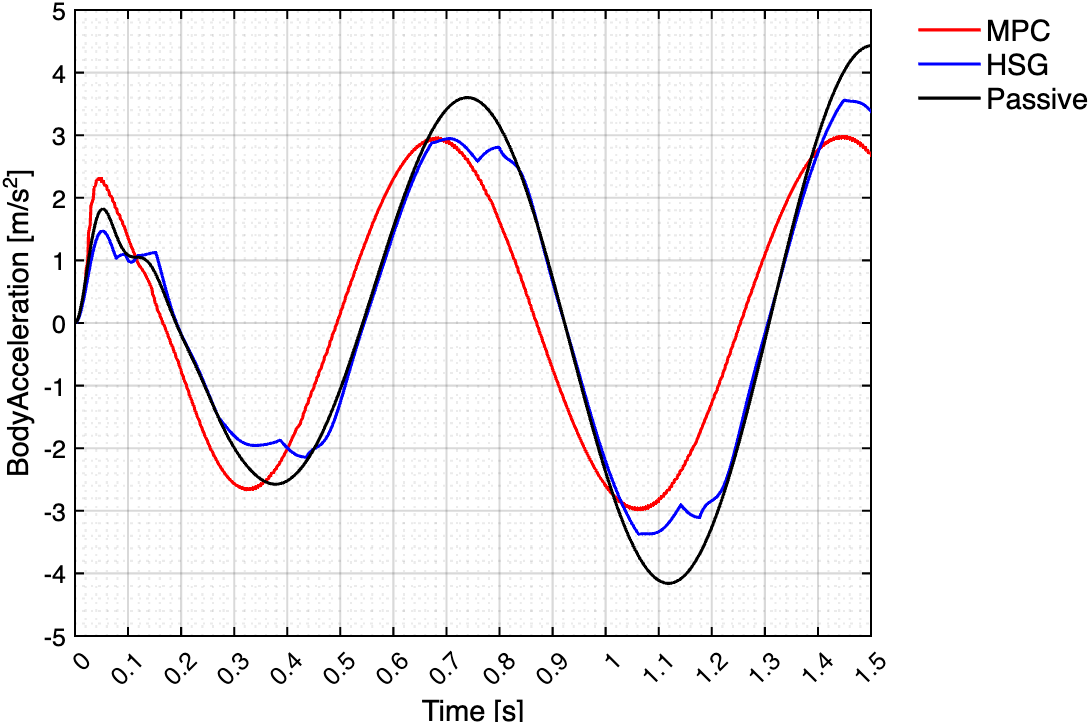
\includegraphics[width=0.75\linewidth]{Results/Graphs/Controller Comparison/BA13.png}
    \caption{Body Acceleration on sinusoidal road profile of frequency = 1.3Hz}
    \label{fig:BAAct13}
\end{figure}
\begin{figure}[H]
    \centering
    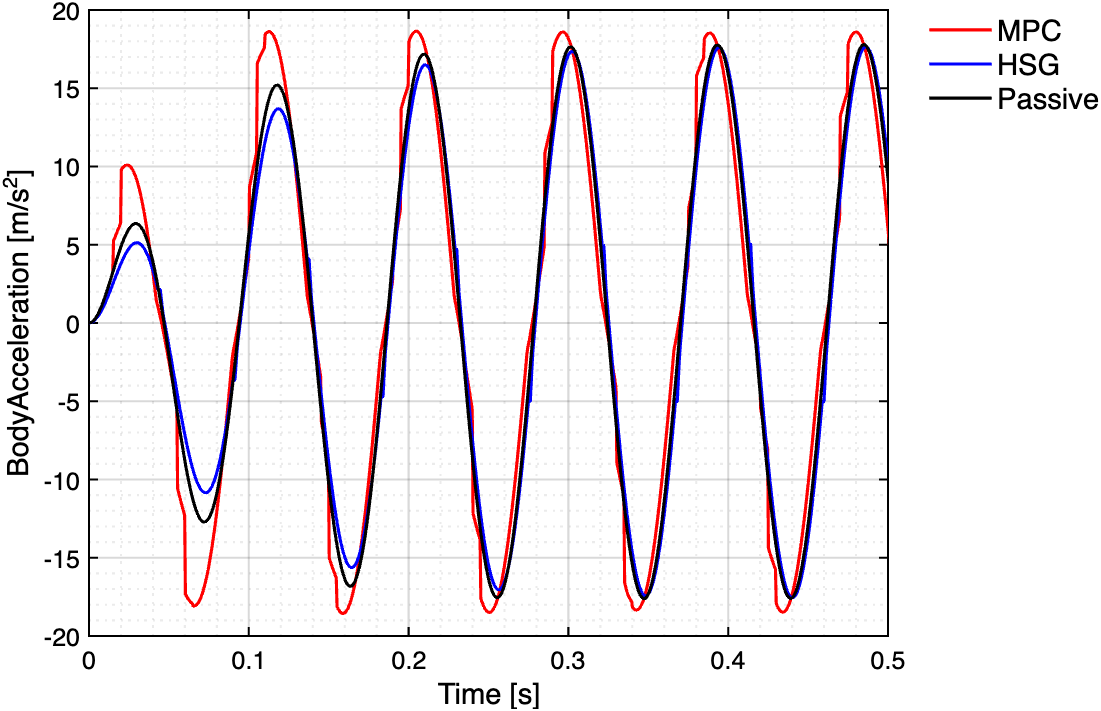
\includegraphics[width=0.75\linewidth]{Results/Graphs/Controller Comparison/BA109.png}
    \caption{Body Acceleration on sinusoidal road profile of frequency = 10.9Hz}
    \label{fig:BAAct109}
\end{figure}
\begin{figure}[H]
    \centering
    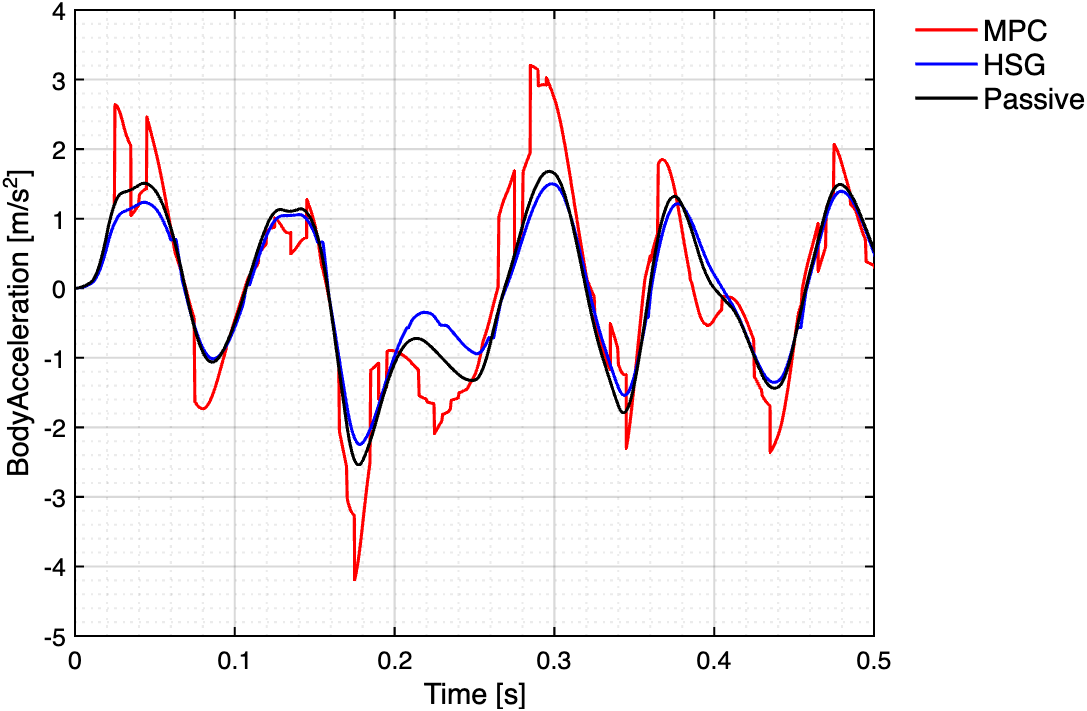
\includegraphics[width=0.75\linewidth]{Results/Graphs/Controller Comparison/BABH.png}
    \caption{Body Acceleration on class B road at 120km/h}
    \label{fig:BAActBH}
\end{figure}
\begin{figure}[H]
    \centering
    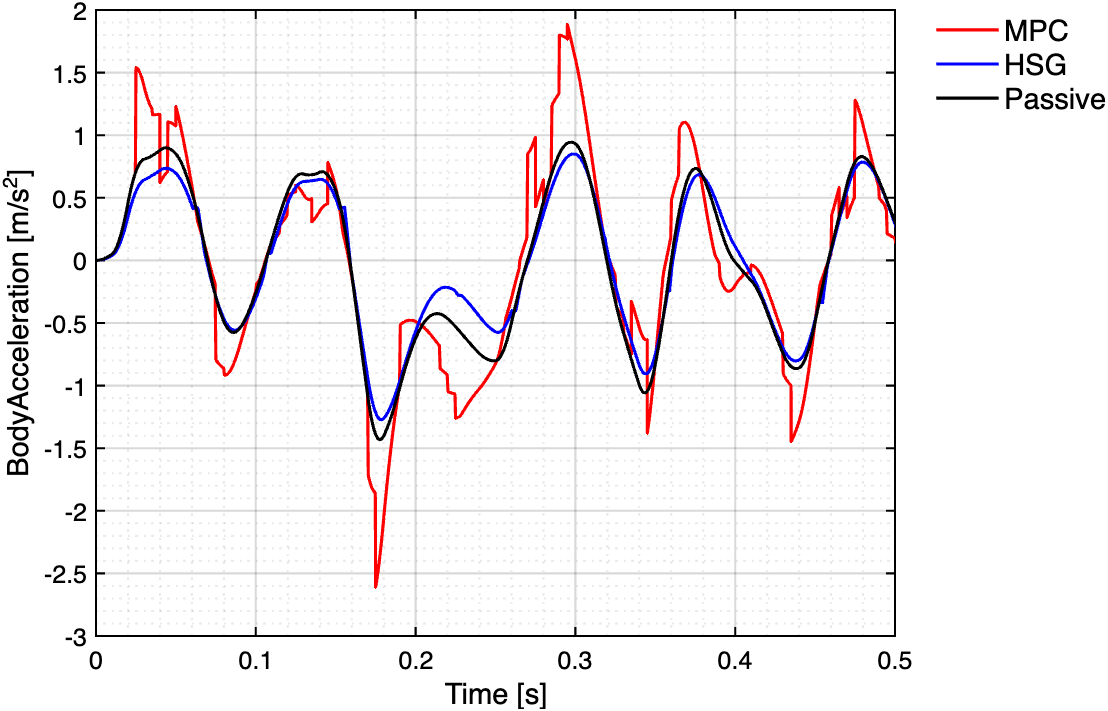
\includegraphics[width=0.75\linewidth]{Results/Graphs/Controller Comparison/BABL.png}
    \caption{Body Acceleration on class B road at 40km/h}
    \label{fig:BAActBL}
\end{figure}
\begin{figure}[H]
    \centering
    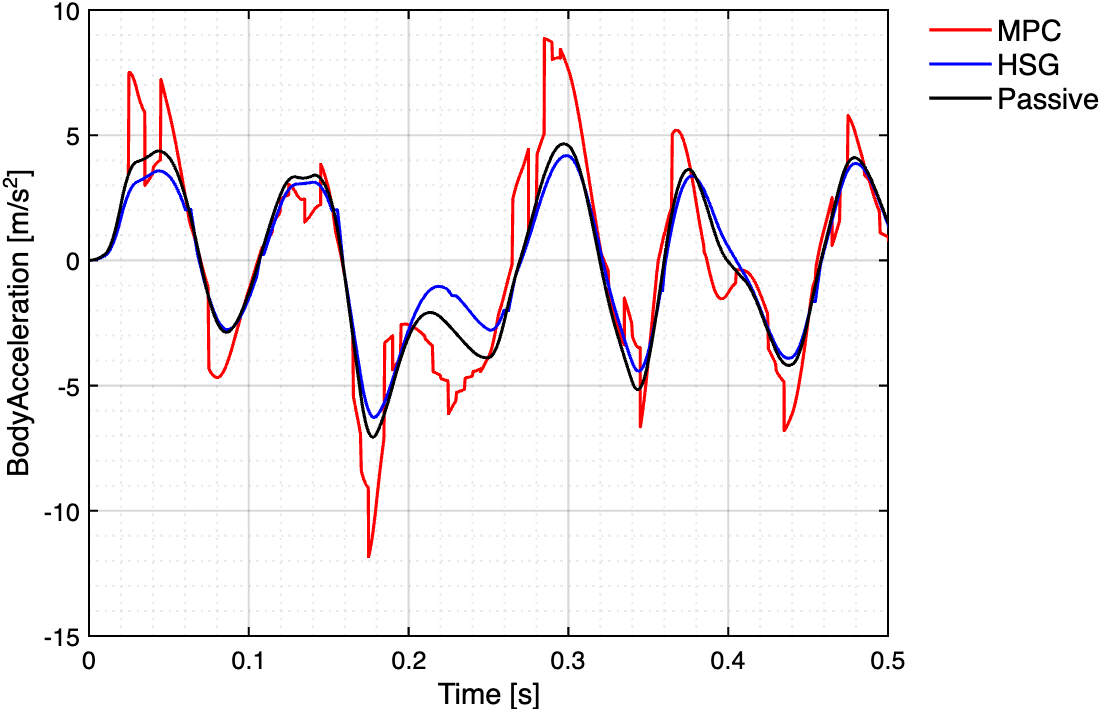
\includegraphics[width=0.75\linewidth]{Results/Graphs/Controller Comparison/BADH.png}
    \caption{Body Acceleration on class D road at 60km/h}
    \label{fig:BAActDH}
\end{figure}
\begin{figure}[H]
    \centering
    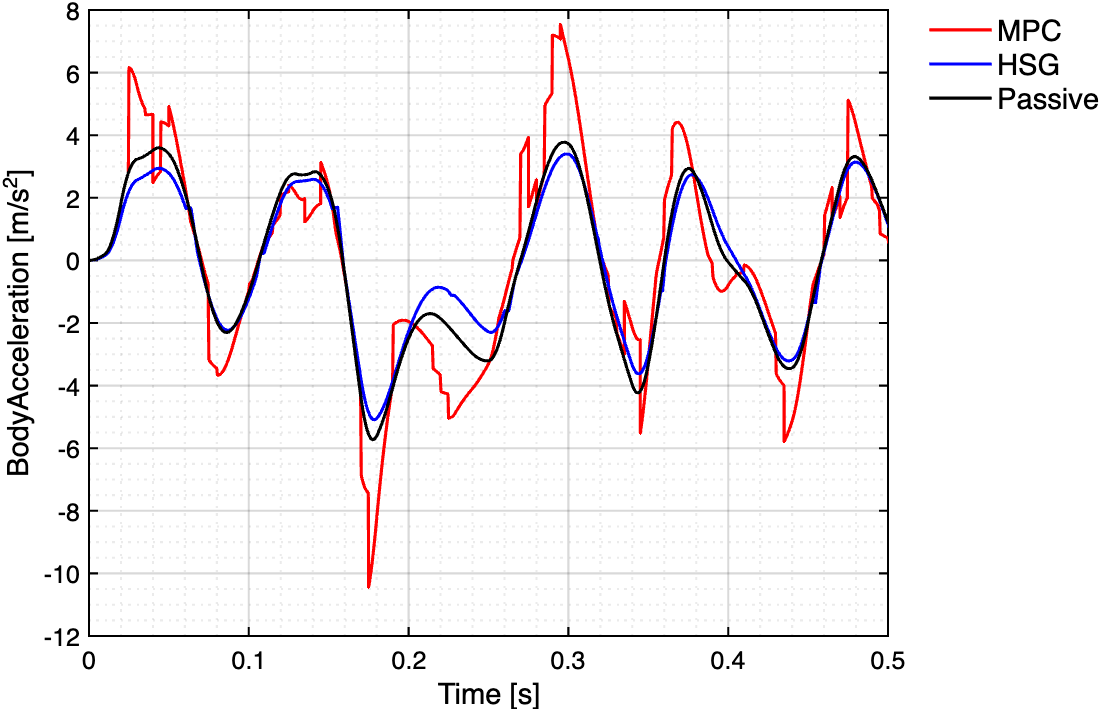
\includegraphics[width=0.75\linewidth]{Results/Graphs/Controller Comparison/BADL.png}
    \caption{Body Acceleration on class D road at 40km/h}
    \label{fig:BAActDL}
\end{figure}

The closed-loop metrics demonstrate clear strategic differences between the controllers regarding occupant comfort. At the 1.3~Hz sprung mass resonance, the MPC architecture yields a $15.2\%$ reduction in body acceleration RMS compared to the passive baseline. The HSG controller exhibits a minor increase in body acceleration RMS ($+2.5\%$). Under stochastic ISO road conditions, the HSG controller favors occupant comfort, reducing body acceleration RMS by approximately $16.0\%$ compared to the passive suspension. The adaptive MPC scheduler, focused on road holding in these specific test states, yields a stiffer ride, increasing body acceleration RMS by $\sim33\%$ relative to the passive baseline.

\begin{table}[H]
    \centering
    \caption{Closed-Loop Performance: Body Acceleration}
    \label{tab:cl_ba_metrics}
    \renewcommand{\arraystretch}{1.2}
    \begin{tabular}{lccc}
        \toprule
        \textbf{Scenario} & \textbf{Passive RMS} [m/s$^2$] & \textbf{HSG RMS} [m/s$^2$] & \textbf{MPC RMS} [m/s$^2$] \\
        \midrule
        1.3 Hz Sine      & 2.45  & 2.51  (+2.5\%)  & 2.08  (-15.2\%) \\
        10.9 Hz Sine     & 12.17 & 12.01 (-1.3\%)  & 12.42 (+2.0\%) \\
        Class B, 120 km/h& 1.12  & 0.94  (-16.0\%) & 1.50  (+34.3\%) \\
        Class B, 40 km/h & 0.65  & 0.55  (-16.0\%) & 0.86  (+33.0\%) \\
        Class D, 60 km/h & 3.18  & 2.67  (-16.0\%) & 4.25  (+33.8\%) \\
        Class D, 40 km/h & 2.60  & 2.18  (-16.0\%) & 3.46  (+33.0\%) \\
        \bottomrule
    \end{tabular}
\end{table}

\subsection{Tyre Dynamic Load}
\begin{figure}[H]
    \centering
    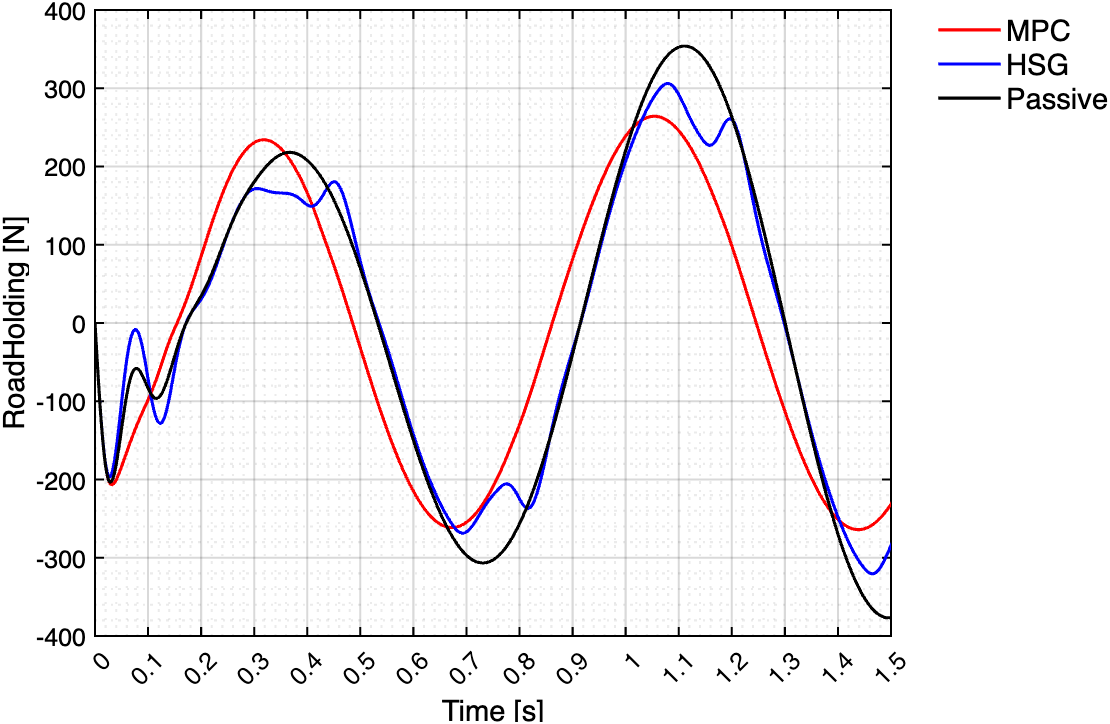
\includegraphics[width=0.75\linewidth]{Results/Graphs/Controller Comparison/RH13.png}
    \caption{Tyre Dynamic Load on sinusoidal road profile of frequency = 1.3Hz}
    \label{fig:RHAct13}
\end{figure}
\begin{figure}[H]
    \centering
    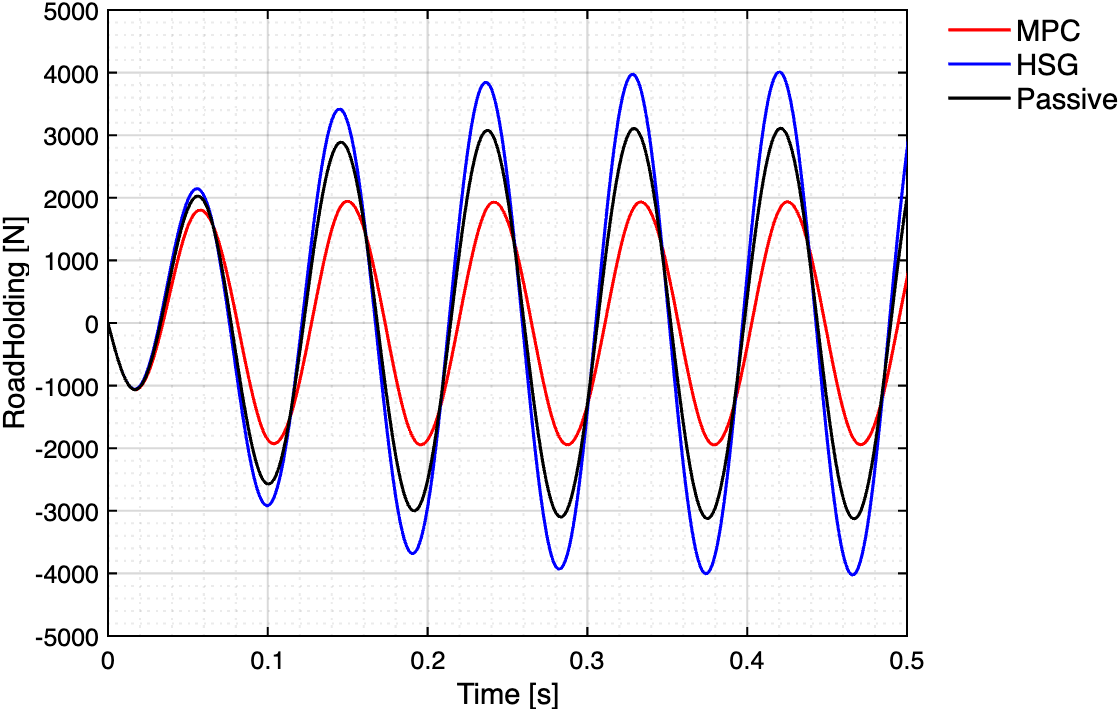
\includegraphics[width=0.75\linewidth]{Results/Graphs/Controller Comparison/RH109.png}
    \caption{Tyre Dynamic Load on sinusoidal road profile of frequency = 10.9Hz}
    \label{fig:RHAct109}
\end{figure}
\begin{figure}[H]
    \centering
    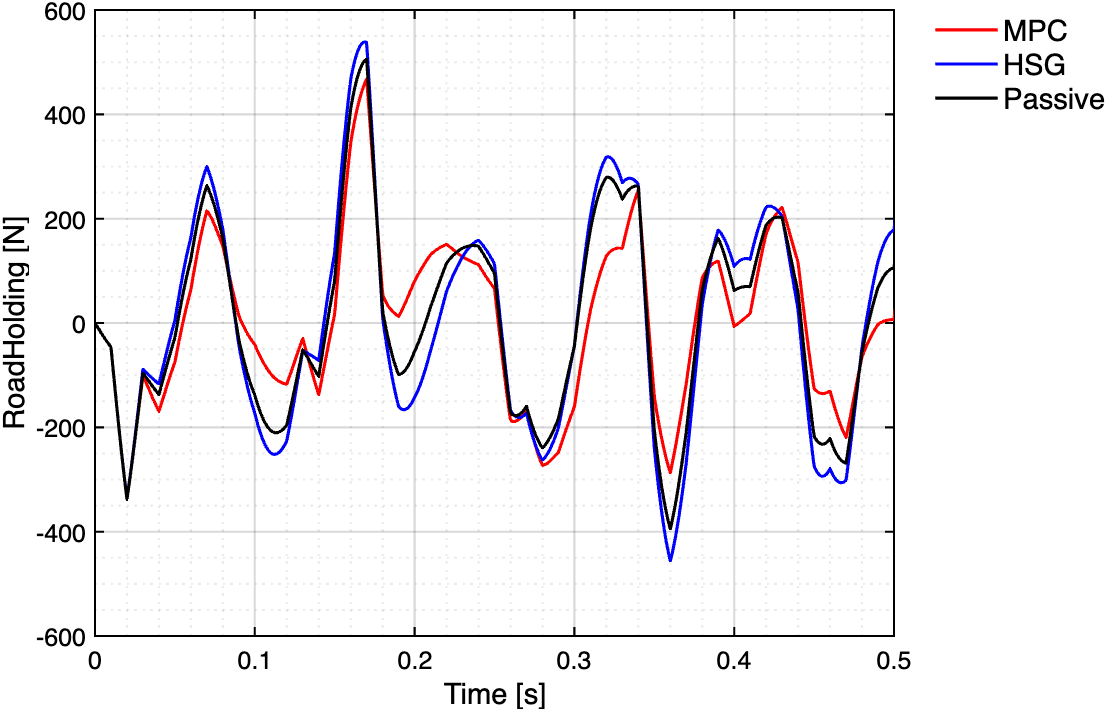
\includegraphics[width=0.75\linewidth]{Results/Graphs/Controller Comparison/RHBH.png}
    \caption{Tyre Dynamic Load on class B road at 120km/h}
    \label{fig:RHActBH}
\end{figure}
\begin{figure}[H]
    \centering
    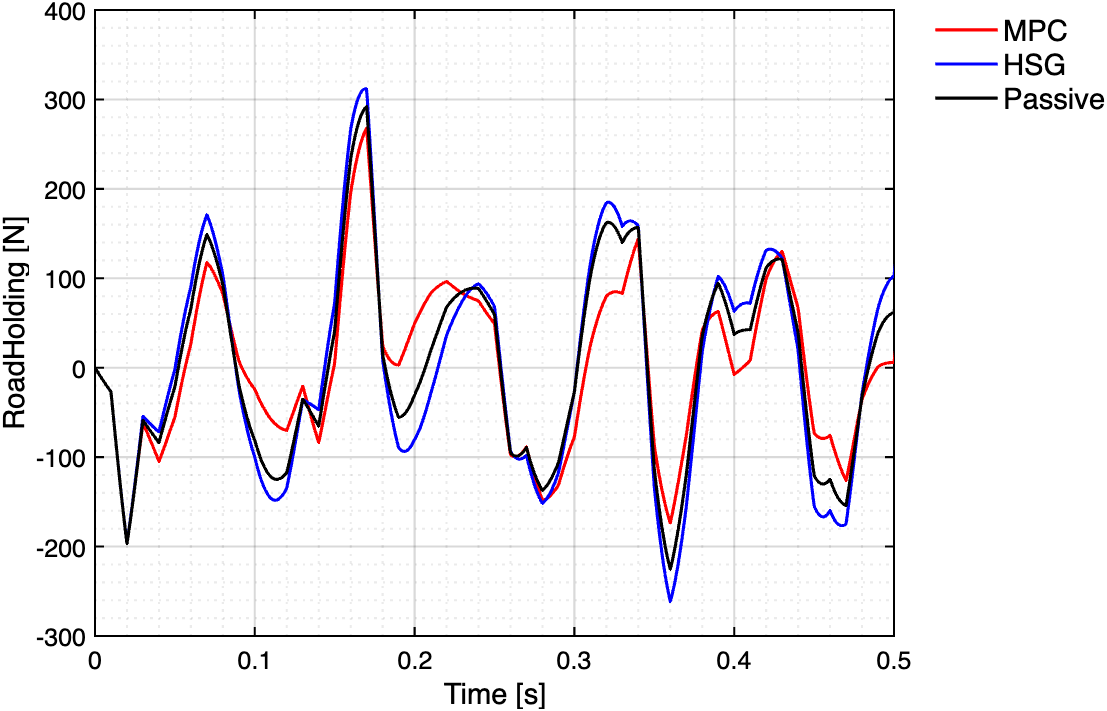
\includegraphics[width=0.75\linewidth]{Results/Graphs/Controller Comparison/RHBL.png}
    \caption{Tyre Dynamic Load on class B road at 40km/h}
    \label{fig:RHActBL}
\end{figure}
\begin{figure}[H]
    \centering
    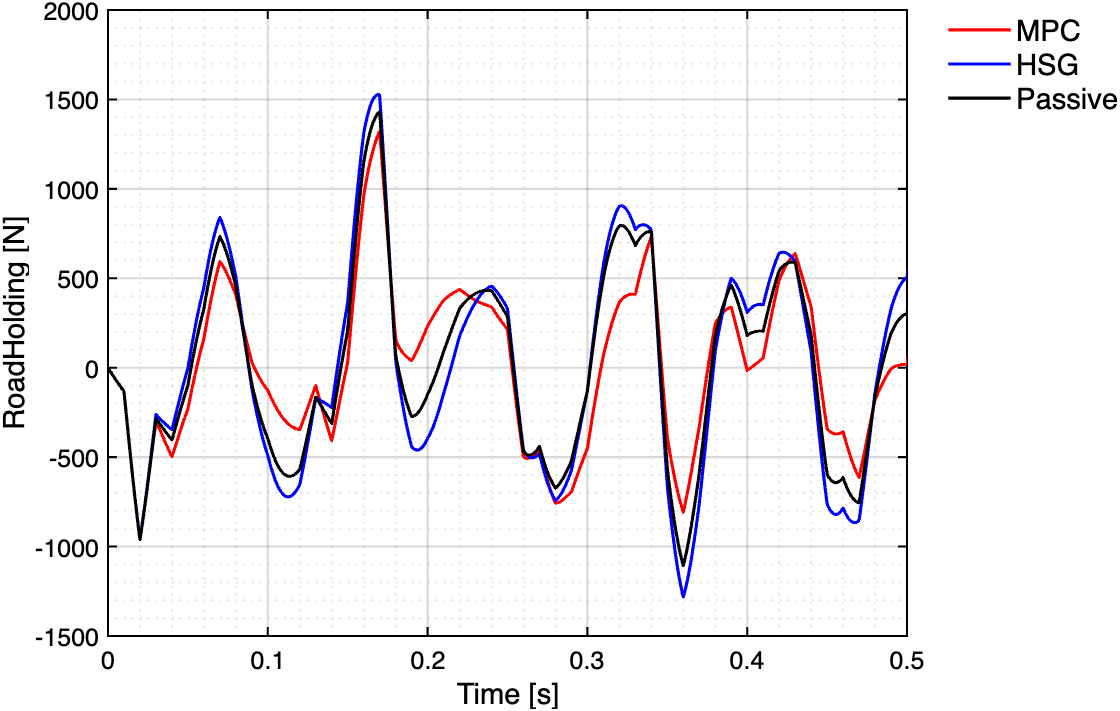
\includegraphics[width=0.75\linewidth]{Results/Graphs/Controller Comparison/RHDH.png}
    \caption{Tyre Dynamic Load on class D road at 60km/h}
    \label{fig:RHActDH}
\end{figure}
\begin{figure}[H]
    \centering
    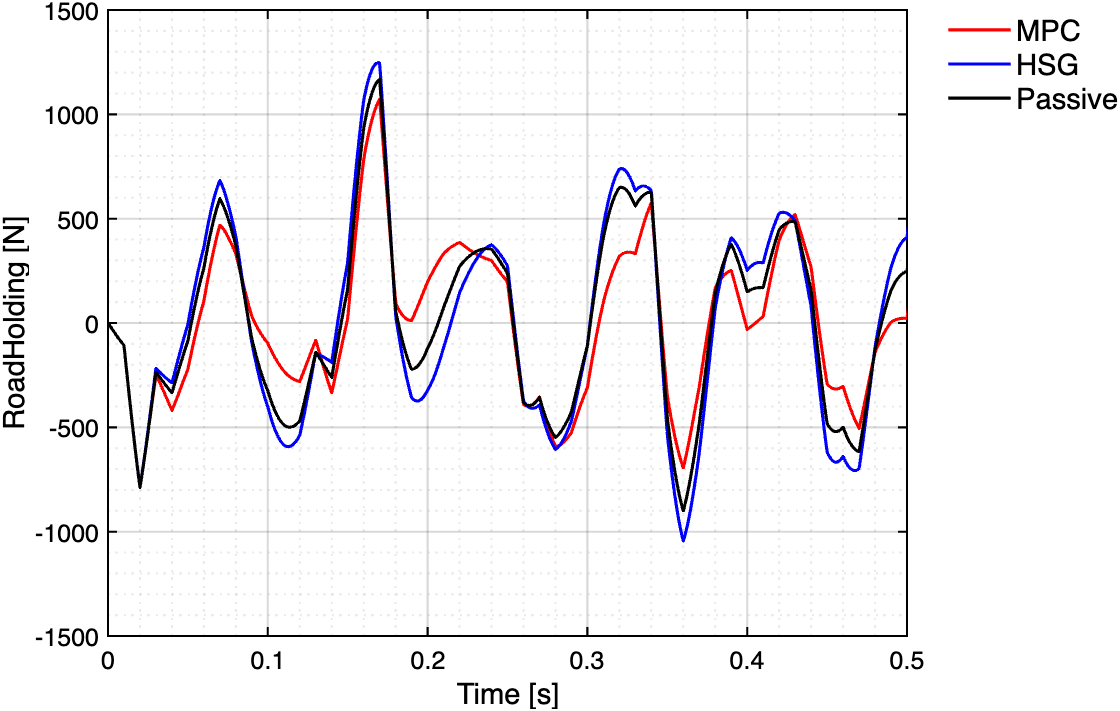
\includegraphics[width=0.75\linewidth]{Results/Graphs/Controller Comparison/RHDL.png}
    \caption{Tyre Dynamic Load on class D road at 40km/h}
    \label{fig:RHActDL}
\end{figure}

The road-holding capabilities heavily favor the MPC algorithm. During the 10.9~Hz unsprung mass resonance, the MPC heavily prioritizes wheel tracking, resulting in a substantial $36.7\%$ reduction in tyre dynamic load RMS over the passive system, whereas the HSG records a $27.7\%$ increase. On stochastic roads, the MPC consistently stiffens the suspension to improve road holding (reducing tyre dynamic load RMS by $7.2\%$ to $8.0\%$), while the HSG incurs a penalty of a $9.1\%$ increase in tyre dynamic load RMS, marginally reducing tyre-road contact.

\begin{table}[H]
    \centering
    \caption{Closed-Loop Performance: Tyre Dynamic Load}
    \label{tab:cl_rh_metrics}
    \renewcommand{\arraystretch}{1.2}
    \begin{tabular}{lccc}
        \toprule
        \textbf{Scenario} & \textbf{Passive RMS} [N] & \textbf{HSG RMS} [N] & \textbf{MPC RMS} [N] \\
        \midrule
        1.3 Hz Sine      & 210.8  & 216.1   (+2.6\%)  & 184.8   (-12.3\%) \\
        10.9 Hz Sine     & 2143.8 & 2736.7  (+27.7\%) & 1356.8  (-36.7\%) \\
        Class B, 120 km/h& 176.1  & 192.2   (+9.1\%)  & 163.5   (-7.2\%)  \\
        Class B, 40 km/h & 101.9  & 111.2   (+9.1\%)  & 93.7    (-8.0\%)  \\
        Class D, 60 km/h & 499.0  & 544.4   (+9.1\%)  & 463.1   (-7.2\%)  \\
        Class D, 40 km/h & 407.5  & 444.7   (+9.1\%)  & 374.8   (-8.0\%)  \\
        \bottomrule
    \end{tabular}
\end{table}

\subsection{Power}
\begin{figure}[H]
    \centering
    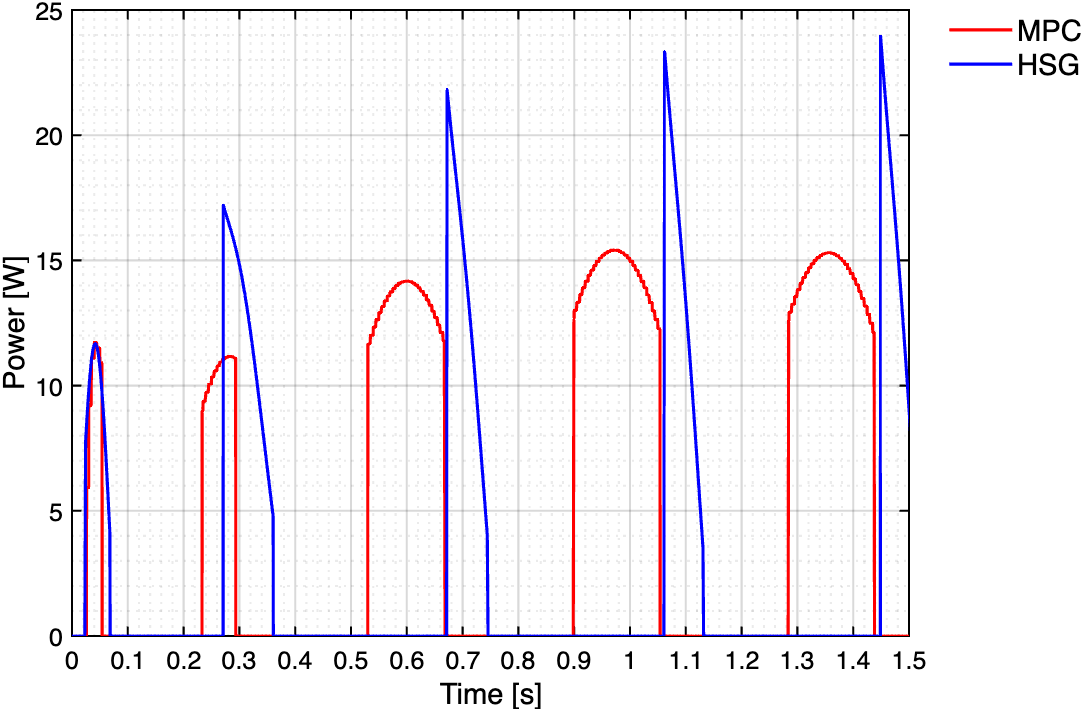
\includegraphics[width=0.75\linewidth]{Results/Graphs/Controller Comparison/P13.png}
    \caption{Power on sinusoidal road profile of frequency = 1.3Hz}
    \label{fig:P13}
\end{figure}
\begin{figure}[H]
    \centering
    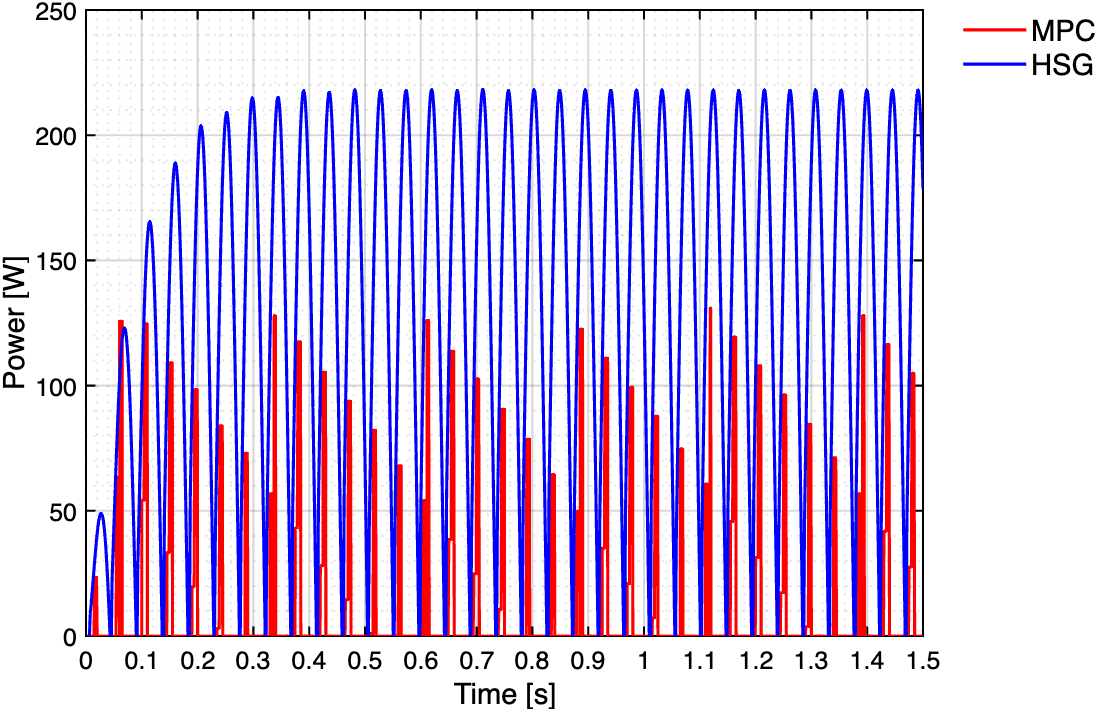
\includegraphics[width=0.75\linewidth]{Results/Graphs/Controller Comparison/P109.png}
    \caption{Power on sinusoidal road profile of frequency = 10.9Hz}
    \label{fig:P109}
\end{figure}
\begin{figure}[H]
    \centering
    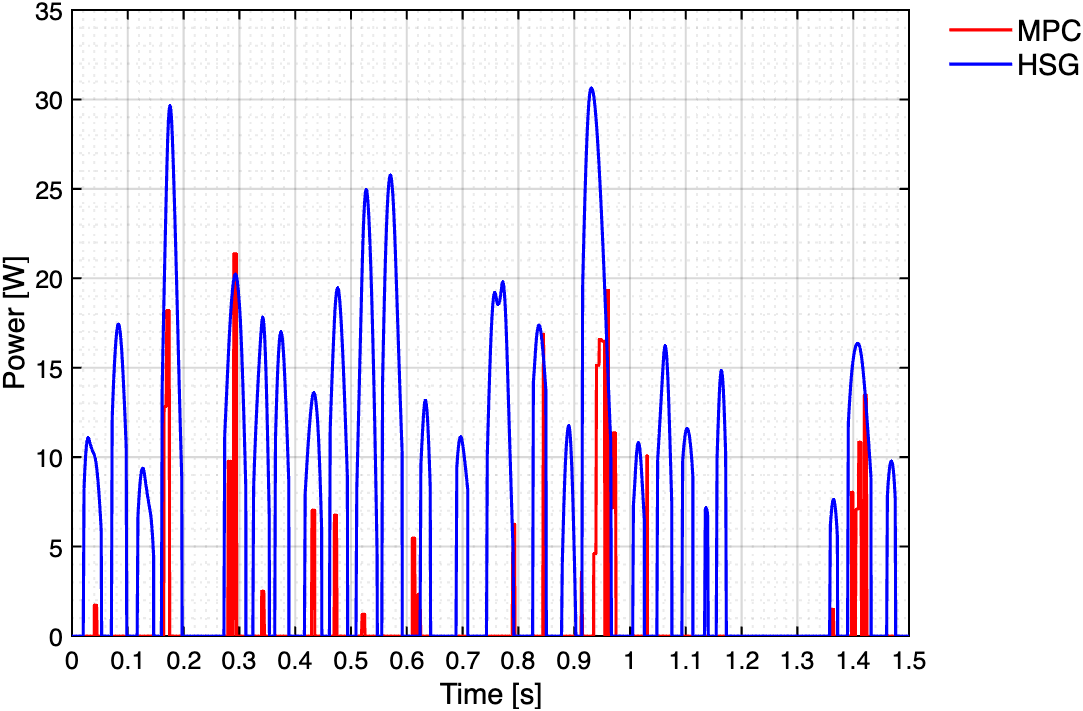
\includegraphics[width=0.75\linewidth]{Results/Graphs/Controller Comparison/PBH.png}
    \caption{Power on class B road at 120km/h}
    \label{fig:PBH}
\end{figure}
\begin{figure}[H]
    \centering
    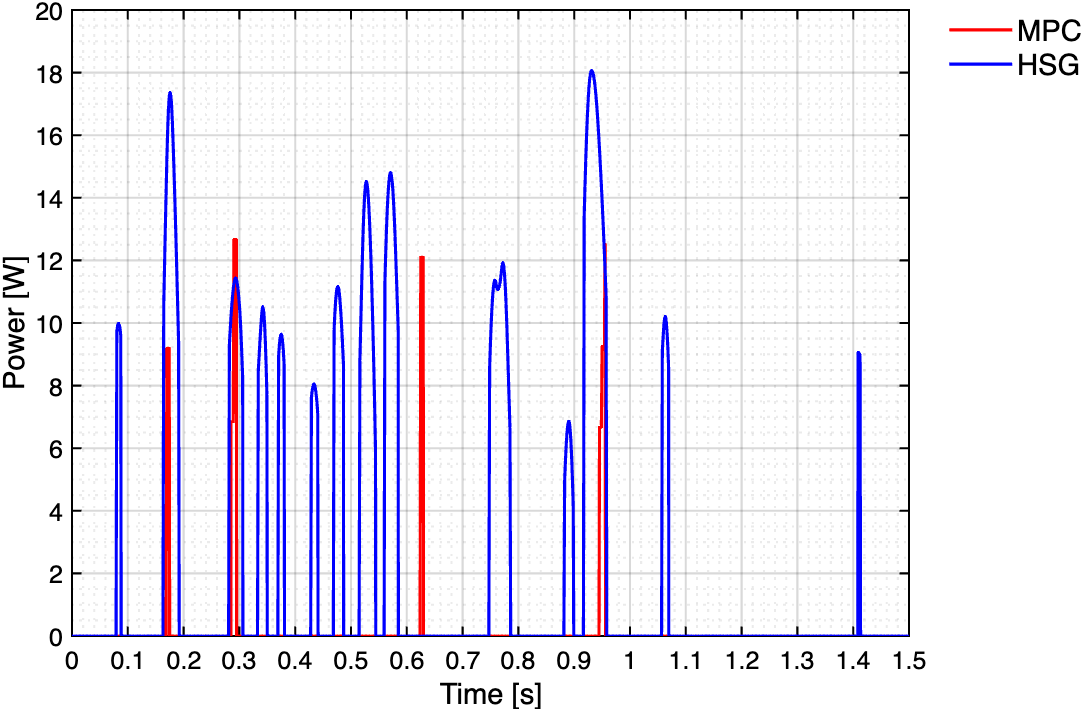
\includegraphics[width=0.75\linewidth]{Results/Graphs/Controller Comparison/PBL.png}
    \caption{Power on class B road at 40km/h}
    \label{fig:PBL}
\end{figure}
\begin{figure}[H]
    \centering
    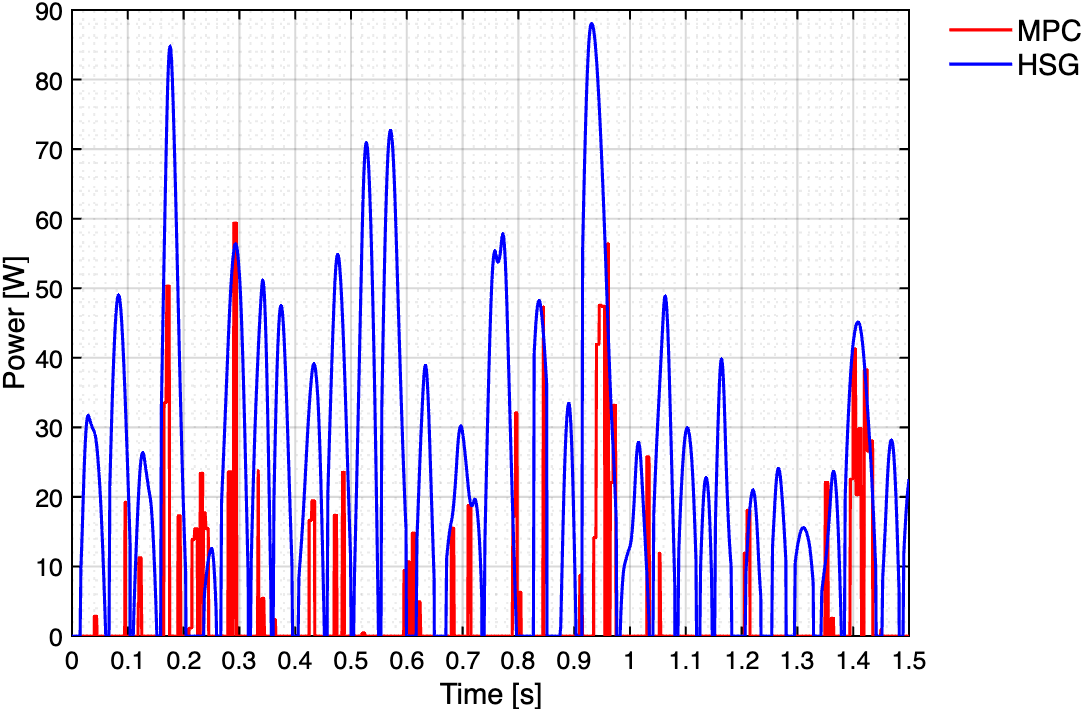
\includegraphics[width=0.75\linewidth]{Results/Graphs/Controller Comparison/PDH.png}
    \caption{Power on class D road at 60km/h}
    \label{fig:PDH}
\end{figure}
\begin{figure}[H]
    \centering
    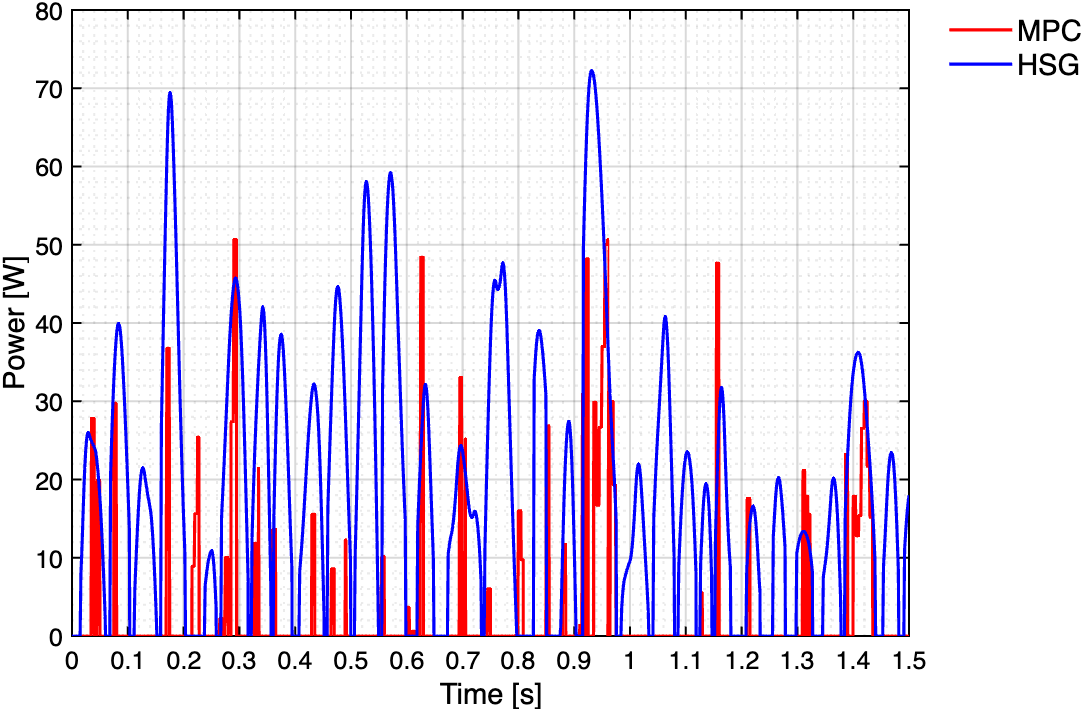
\includegraphics[width=0.75\linewidth]{Results/Graphs/Controller Comparison/PDL.png}
    \caption{Power on class D road at 40km/h}
    \label{fig:PDL}
\end{figure}

The power regeneration metrics reflect the controllers' respective dynamic behaviors. At 1.3~Hz, the MPC extracts $8.8\text{ W}$ (RMS) while simultaneously improving chassis isolation, whereas the HSG yields only $6.5\text{ W}$. At 10.9~Hz, the HSG records an excessively high generated power of $148.4\text{ W}$, which is a parasitic symptom of its failure to suppress massive, uncontrolled wheel oscillations. The MPC intentionally dampens this resonance to secure the tyre, extracting a controlled $34.1\text{ W}$. Across the stochastic roads, the MPC harvests conservatively but consistently (e.g., $10.1\text{ W}$ on Class D at 60~km/h), explicitly avoiding the unsafe resonance exploitation that inflates the HSG's high-frequency power figures.

\begin{table}[H]
    \centering
    \caption{Closed-Loop Performance: RMS Power Generation}
    \label{tab:cl_power_metrics}
    \renewcommand{\arraystretch}{1.2}
    \begin{tabular}{lcc}
        \toprule
        \textbf{Scenario} & \textbf{HSG Power RMS} [W] & \textbf{MPC Power RMS} [W] \\
        \midrule
        1.3 Hz Sine      & 6.5   & 8.8  \\
        10.9 Hz Sine     & 148.4 & 34.1 \\
        Class B, 120 km/h& 10.7  & 3.0  \\
        Class B, 40 km/h & 5.1   & 1.4  \\
        Class D, 60 km/h & 31.6  & 10.1 \\
        Class D, 40 km/h & 25.8  & 9.8  \\
        \bottomrule
    \end{tabular}
\end{table}